\documentclass{standalone}

\usepackage{graphicx}
\usepackage[usenames,dvipsnames]{xcolor}

\usepackage{tikz}
\usetikzlibrary{shapes,calc}

\usepackage{fontspec}
\setmainfont[Scale=1]{Linux Libertine}

\begin{document}
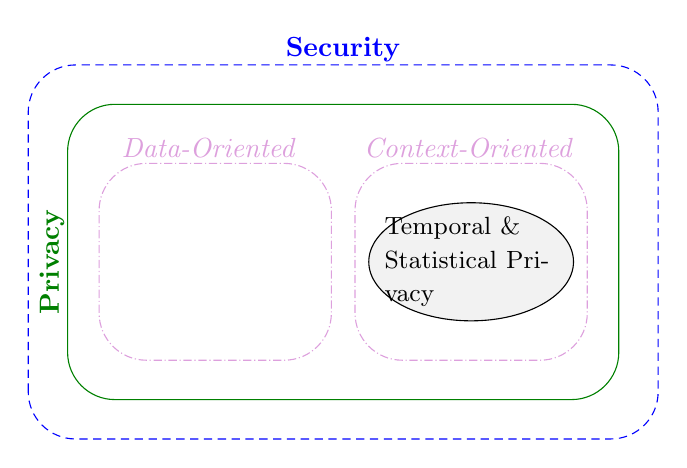
\begin{tikzpicture}

\draw[rounded corners=6mm,Blue,densely dashed](0,.25)rectangle(8,5);
\node at(4,5.2)[Blue]{\textbf{Security}};

\draw[rounded corners=6mm,Green](.5,.75)rectangle(7.5,4.5);
\node at(.3,2.5)[rotate=90,Green]{\textbf{Privacy}};


\draw[rounded corners=6mm,Plum,densely dashdotted](.9,1.25)rectangle(3.85,3.75);
\draw[rounded corners=6mm,Plum,densely dashdotted](4.15,1.25)rectangle(7.1,3.75);
\node at(2.3,3.95)[,Plum]{\textit{Data-Oriented}};
\node at(5.6,3.95)[,Plum]{\textit{Context-Oriented}};

\draw[black,fill=gray!10](5.625,2.5)ellipse(1.3cm and .75cm)node[text width=2.2cm]{\small Temporal \& Statistical Privacy};


\end{tikzpicture}
\end{document}
